\documentclass[10pt,landscape,a4paper]{article}
%\usepackage[utf8]{inputenc}
%\usepackage[ngerman]{babel}
\usepackage[normalem]{ulem}
\usepackage{tikz}
\usetikzlibrary{shapes,positioning,arrows,fit,calc,graphs,graphs.standard}
\usepackage[nosf]{kpfonts}
\usepackage[t1]{sourcesanspro}
%\usepackage[lf]{MyriadPro}
%\usepackage[lf,minionint]{MinionPro}
\usepackage{multicol}
\usepackage{wrapfig}
\usepackage[top=0mm,bottom=1mm,left=0mm,right=1mm]{geometry}
\usepackage[framemethod=tikz]{mdframed}
\usepackage{microtype}
%\usepackage{physics}
\usepackage{tabularx}
\usepackage{hhline}
\usepackage{makecell}
\usepackage{mathtools}
\usepackage{amssymb}
\usepackage{mathabx}

\usepackage{listings}

\DeclarePairedDelimiter{\ceil}{\lceil}{\rceil}

\newcommand\codeblue[1]{\textcolor{blue}{\code{#1}}}

\usepackage{lastpage}
\usepackage{datetime}
\yyyymmdddate
\renewcommand{\dateseparator}{-}
\let\bar\overline

\definecolor{myblue}{cmyk}{1,.72,0,.38}

\def\firstcircle{(0,0) circle (1.5cm)}
\def\secondcircle{(0:2cm) circle (1.5cm)}

\colorlet{circle edge}{myblue}
\colorlet{circle area}{myblue!5}

\tikzset{filled/.style={fill=circle area, draw=circle edge, thick},
outline/.style={draw=circle edge, thick}}

\pgfdeclarelayer{background}
\pgfsetlayers{background,main}

%\everymath\expandafter{\the\everymath \color{myblue}}
%\everydisplay\expandafter{\the\everydisplay \color{myblue}}


\renewcommand{\baselinestretch}{.8}
\pagestyle{empty}

\global\mdfdefinestyle{header}{%
  linecolor=gray,linewidth=1pt,%
  leftmargin=0mm,rightmargin=0mm,skipbelow=0mm,skipabove=0mm,
}

\newcommand{\header}{
  \begin{mdframed}[style=header]
    \footnotesize
    \sffamily
    CS2102 Finals v1.1 (\today)\\
    by~Dumboiroy,~page~\thepage~of~\pageref{LastPage}
  \end{mdframed}
}

\let\counterwithout\relax
\let\counterwithin\relax
\usepackage{chngcntr}

\usepackage{verbatim}

\usepackage{etoolbox}
\makeatletter
\preto{\@verbatim}{\topsep=0pt \partopsep=0pt }
\makeatother

\counterwithin*{equation}{section}
\counterwithin*{equation}{subsection}
\usepackage{enumitem}
\newlist{legal}{enumerate}{10}
\setlist[legal]{label*=\arabic*.,leftmargin=2.5mm}
\setlist[itemize]{leftmargin=3mm}
\setlist[enumerate]{leftmargin=3.5mm}
\setlist{nosep}
\usepackage{minted}

\def\code#1{\texttt{#1}}

\newenvironment{descitemize} % a mixture of description and itemize
{\begin{description}[leftmargin=*,before=\let\makelabel\descitemlabel]}
{\end{description}}

\newcommand{\descitemlabel}[1]{%
  \textbullet\ \textbf{#1}%
}
\makeatletter



\renewcommand{\section}{\@startsection{section}{1}{0mm}%
  {.2ex}%
  {.2ex}%x
{\color{myblue}\sffamily\small\bfseries}}
\renewcommand{\subsection}{\@startsection{subsection}{1}{0mm}%
  {.2ex}%
  {.2ex}%x
{\sffamily\bfseries}}
\renewcommand{\subsubsection}{\@startsection{subsubsection}{1}{0mm}%
  {.2ex}%
  {.2ex}%x
{\rmfamily\bfseries}}

\global\let\tikz@ensure@dollar@catcode=\relax

\def\mathcolor#1#{\@mathcolor{#1}}
\def\@mathcolor#1#2#3{%
  \protect\leavevmode
  \begingroup
  \color#1{#2}#3%
  \endgroup
}

\makeatother
\setlength{\parindent}{0pt}

\setminted{tabsize=2, breaklines}
% Remove belowskip of minted
\setlength\partopsep{-\topsep}

\newcolumntype{a}{>{\hsize=1.5\hsize}X}
% \newcolumntype{b}{>{\hsize=.25\hsize}X}

\setlength\columnsep{1.5pt}
\setlength\columnseprule{0.1pt}

\begin{document}
\setlength{\abovedisplayskip}{0pt}
\setlength{\belowdisplayskip}{0pt}

% \header

\scriptsize
\begin{multicols*}{4}
  \header
  \raggedcolumns
  \section{Creating and Populating Tables}
  \begin{itemize}
    \item Point 1
    \item Point 2
  \end{itemize}

  \section{Simple Queries}
  \begin{itemize}
    \item Point 1
    \item Point 2
  \end{itemize}

  \section{Aggregate Queries}
  \begin{itemize}
    \item Point 1
    \item Point 2
  \end{itemize}

  \section{Entity-Relationship Model}

  \subsection{Entity Sets}
  \begin{minipage}{0.75\linewidth}
    \begin{itemize}
      \item Identifiable things grouped into sets
      \item Diagram: named box
      \item All entities in set have same attributes, different values
    \end{itemize}
  \end{minipage}
  \hfill
  \begin{minipage}{0.2\linewidth}
    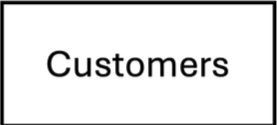
\includegraphics[width=\linewidth]{entity-sets-example}
  \end{minipage}

  \subsection{Attributes}
  % \begin{minipage}{0.6\linewidth}
  \begin{itemize}
    \item Value-oriented: atomic types (INTEGER, TEXT, etc.)
    \item Diagram: circle with name outside
  \end{itemize}
  \begin{itemize}
    \item Simple: single attribute $\Rightarrow$ circle
    \item Derived: computed from others $\Rightarrow$ dashed line (e.g., age from date\_of\_birth)
  \end{itemize}
  % \end{minipage}
  % \hfill
  % \begin{minipage}{0.35\linewidth}
  %   \includegraphics[width=\linewidth]{attributes-types}
  % \end{minipage}

  \subsection{Identifiers}
  \begin{minipage}{0.5\linewidth}
    \begin{itemize}
      \item 1 or more attributes identify entity uniquely
    \end{itemize}
    \begin{itemize}
      \item Single: black circle on attribute
      \item Composite: connected black circles (e.g., name + version)
    \end{itemize}
  \end{minipage}
  \hfill
  \begin{minipage}{0.45\linewidth}
    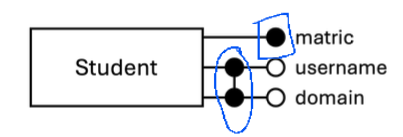
\includegraphics[width=\linewidth]{identifiers-candidate-keys}
  \end{minipage}
  \begin{itemize}
    \item Candidate Key: all minimal sets identifying entity
    \item Property: $\geq 1$ candidate key per entity set
  \end{itemize}
  \begin{itemize}
    \item Minimality condition: cannot remove any attribute without losing identification
    \item Minimal $\neq$ minimum (local vs.\ global)
  \end{itemize}

  \section*{Relationships}
  \subsection{Relationship Sets}
  % \begin{minipage}{0.6\linewidth}
  \begin{itemize}
    \item Associates $\geq 2$ entities (typically 2)
    \item No duplicates: set property
    \item Diagram: named diamond
    \item Description uses verbs (download, refers, supervise)
  \end{itemize}
  % \end{minipage}
  % \hfill
  % \begin{minipage}{0.35\linewidth}
  %   \includegraphics[width=\linewidth]{relationships-binary}
  % \end{minipage}

  \subsection{Relationship Attributes}
  \begin{itemize}
    \item Not distinguished by own attributes
    \item Identified by: participating entities' identifiers
    \item Dependent on entities $\Rightarrow$ attributes are entity-dependent
  \end{itemize}

  \subsection{Same Entity Set Relationships}
  \begin{minipage}{0.7\linewidth}
    \begin{itemize}
      \item Associates entities from same set
      \item Participation roles: named labels (e.g., referee $\leftrightarrow$ referrer)
      \item Rule: participation can always be named even across different entity sets
    \end{itemize}
  \end{minipage}
  \hfill
  \begin{minipage}{0.25\linewidth}
    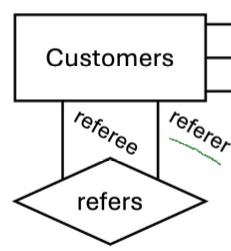
\includegraphics[width=\linewidth]{same-entity-relationship}
  \end{minipage}

  \subsection{n-ary Relationships}
  \begin{minipage}{0.4\linewidth}
    \begin{itemize}
      \item Relate $\geq 2$ entity sets
      \item All participation mandatory: no NULL allowed
      \item Still a set: no duplicates
    \end{itemize}
  \end{minipage}
  \hfill
  \begin{minipage}{0.55\linewidth}
    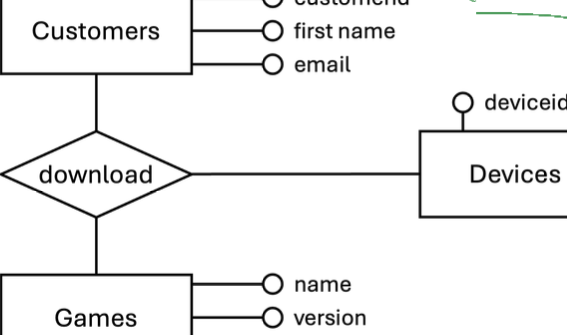
\includegraphics[width=\linewidth]{nary-relationship}
  \end{minipage}

  \subsection{Relationship Identifiers}
  % \begin{minipage}{0.6\linewidth}
  \begin{itemize}
    \item Identified by: participating entities only
    \item Rule: NO black circle on relationship attribute
    \item Invalid: black circle on deviceid $\Rightarrow$ violates uniqueness (duplicate downloads)
    \item Solution: promote attribute to entity set (Devices) $\Rightarrow$ allows multiple same-game downloads per device
  \end{itemize}
  % \end{minipage}
  \hfill
  % \begin{minipage}{0.35\linewidth}
  %   \includegraphics[width=\linewidth]{relationship-identifiers-valid-invalid}
  % \end{minipage}

  \section*{Aggregation}
  \begin{minipage}{0.3\linewidth}
    \begin{itemize}
      \item Associate entity set with relationship set
      \item Diagram: wrap relationship in box
      \item Semantics: relationship becomes entity set
      \item Rules: all relationship set constraints apply (no duplicates, participation, etc.)
    \end{itemize}
  \end{minipage}
  \hfill
  \begin{minipage}{0.65\linewidth}
    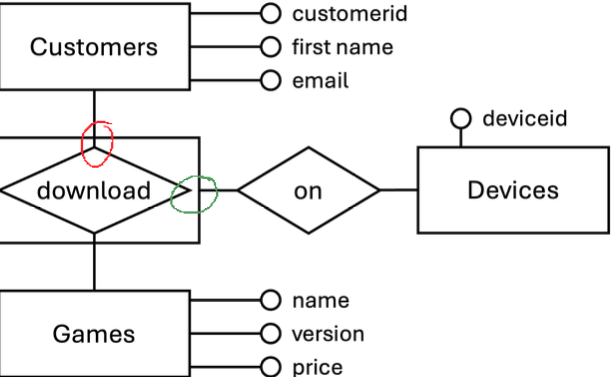
\includegraphics[width=\linewidth]{aggregation-example}
  \end{minipage}

  \section*{Weak Entity Sets}
  \subsection{Partial Identification}
  \begin{minipage}{0.3\linewidth}
    \begin{itemize}
      \item Identified within scope of relationship with dominant entity
      \item Diagram: partial identifier $\rightarrow$ participation of dominant entity
      \item Example: (customerid + appstore) $\rightarrow$ customer unique per app store only
    \end{itemize}
  \end{minipage}
  \hfill
  \begin{minipage}{0.65\linewidth}
    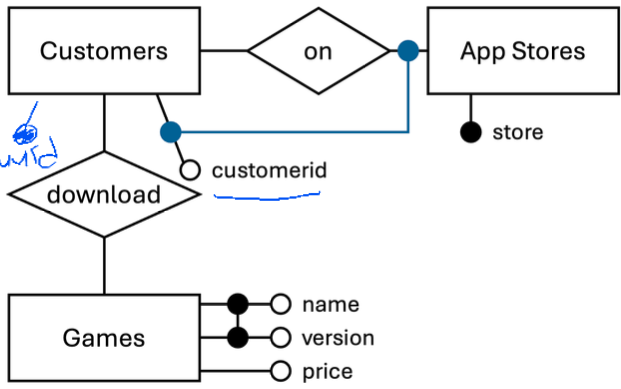
\includegraphics[width=\linewidth]{weak-entity-partial-key}
  \end{minipage}

  \subsection{Terminology}
  \begin{itemize}
    \item Weak entity set: $\geq 1$ partial key
    \item Identifying relationship: enables weak entity identification
    \item Dominant entity set: partner in identifying relationship
    \item Variant: can have both partial and non-partial keys
    \item Variant: partial key can have multiple dominant entities (uncommon)
  \end{itemize}

  \section*{Participation Constraints}
  \subsection{Cardinality Format}
  \begin{itemize}
    \item (min, max) between entity set and relationship
    \item min = 0 (optional) or 1 (mandatory)
    \item max = 1 (one) or n (many)
  \end{itemize}

  \subsection{Classifications (Binary Relations)}
  \begin{itemize}
    \item $(1, \_)$ $\Rightarrow$ mandatory participation
    \item $(0, \_)$ $\Rightarrow$ optional participation
  \end{itemize}
  \begin{itemize}
    \item $(\_,1)$ on both sides $\Rightarrow$ one-to-one
    \item $(\_,1)$ on one, $(\_,n)$ on other $\Rightarrow$ one-to-many
    \item $(\_,n)$ on both sides $\Rightarrow$ many-to-many
  \end{itemize}
  \begin{itemize}
    \item Default (omitted): $(0,n)$
  \end{itemize}

  \subsection{Examples}
  \begin{minipage}{0.3\linewidth}
    \begin{itemize}
      \item Citizens (0,1) has Passports (1,1): one citizen $\Rightarrow$ 0--1 passports, one passport $\Rightarrow$ exactly 1 citizen (one-to-one, optional)
    \end{itemize}
  \end{minipage}
  \hfill
  \begin{minipage}{0.6\linewidth}
    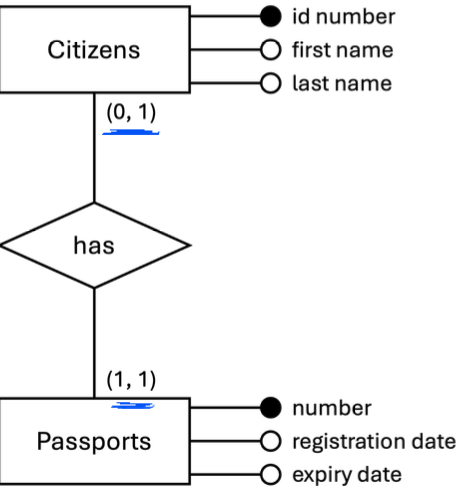
\includegraphics[width=0.6\linewidth]{participation-cardinality-examples}
  \end{minipage}

  \section*{Conversion to Relational Schema}
  \subsection{Rule \#1: Value Sets}
  \begin{itemize}
    \item Value sets $\rightarrow$ domains
    \item ER attributes $\rightarrow$ relation attributes + meaningful type
    \item Default: NOT NULL constraint
    \item Justify every NULL instance (avoid unless necessary)
  \end{itemize}

  \subsection{Rule \#2: Entity Sets}
  \begin{itemize}
    \item Entity sets $\rightarrow$ relations
    \item Attributes $\rightarrow$ relation attributes
    \item Candidate keys $\rightarrow$ PRIMARY KEY + UNIQUE NOT NULL
  \end{itemize}



  \section{Nested Queries}
  \begin{itemize}
    \item Point 1
    \item Point 2
  \end{itemize}

  \section{Relational Algebra}
  \subsection{Relational Algebra Operators}

  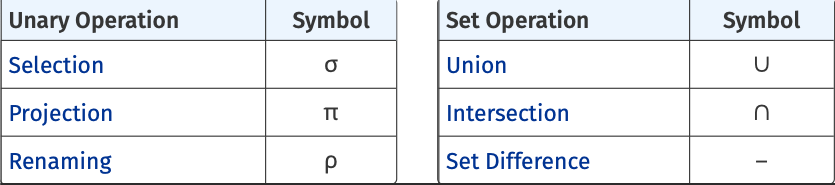
\includegraphics[width=\linewidth]{rel-ops-1}
  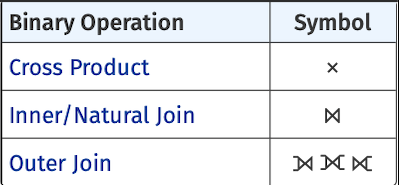
\includegraphics[width=0.5\linewidth]{rel-ops-2}


  \subsection{Notation \& Fundamentals}
  \begin{tabular}{ll}
    $\sigma$  & Selection (WHERE)   \\
    $\pi$     & Projection (SELECT) \\
    $\rho$    & Renaming (AS)       \\
    $\times$  & Cross Product       \\
    $\bowtie$ & Natural Join        \\
    $\cup$    & Union               \\
    $\cap$    & Intersection        \\
    $-$       & Set Difference      \\
  \end{tabular}

  \textbf{Properties:} Sets (no duplicates) • No row order • Column order matters • Tuples immutable

  ---

  \subsection{Unary Operators}

  \subsubsection*{Selection: $\sigma_c(R)$}
  • Filter rows by condition $c$ \\
  • Same columns, fewer rows \\
  • Example: $\sigma_{country='SG'}(customers)$ \\
  • NULL: $\neg(NULL = NULL)$ $\Rightarrow$ row excluded

  \subsubsection*{Projection: $\pi_{[list]}(R)$}
  • Keep columns in specified order \\
  • \textbf{Auto-deduplicates} (set semantics) \\
  • Cannot add/derive columns \\
  • Example: $\pi_{[name, email]}(customers)$ \\
  • $\neq$ SQL SELECT (requires DISTINCT)

  \subsubsection*{Renaming: $\rho(R_1, R_2)$ or $\rho(R, R_2(A \to B))$}
  • Rename relation \& attributes locally \\
  • For self-joins: $\rho(downloads, d_1)$ \\
  • Scope: within query only

  ---

  \subsection{Set Operations}

  \textbf{Requirement:} Union-compatible (same column types/count)

  \begin{tabular}{ll}
    $R \cup S$ & All rows (dedup)       \\
    $R \cap S$ & Only common rows       \\
    $R - S$    & Rows in $R$ not in $S$ \\
  \end{tabular}

  ---

  \subsection{Binary Operators}

  \subsubsection*{Cross Product: $R_1 \times R_2$}
  • Combine each row of $R_1$ with each row of $R_2$ \\
  • Output rows: $n \times m$ \\
  • Usually used with selection: $\sigma_c(R_1 \times R_2)$ \\
  • Expensive for large tables

  \subsubsection*{Inner Join: $R_1 \bowtie_c R_2$}
  • Equivalent: $\sigma_c(R_1 \times R_2)$ \\
  • Only matching rows \\
  • Example: $R_1 \bowtie_{R_1.id = R_2.id} R_2$ \\
  • NULL in join key $\Rightarrow$ no match

  \subsubsection*{Natural Join: $R_1 \bowtie R_2$}
  • Join on common attribute names \\
  • Keeps one copy of common columns \\
  • Common attrs first, then $R_1$ uniques, then $R_2$ uniques \\
  • Pitfall: ambiguous column names

  \subsubsection*{Outer Joins}
  • Left ($\rtimes$): Keep all left rows, NULL for unmatched right \\
  • Right ($\ltimes$): Keep all right rows, NULL for unmatched left \\
  • Full ($\bowtie|$): Keep all rows both sides

  ---

  \subsection{Query Optimization}

  \subsubsection*{Equivalences:}
  1. Push selection down: $\sigma_c(\pi[cols](R)) = \pi[cols](\sigma_c(R))$ \\
  2. Split AND: $\sigma_{A \land B}(R) = \sigma_A(\sigma_B(R))$ \\
  3. Cannot split OR: $\sigma_{A \lor B}$ stays together \\
  4. Reorder joins: Based on table size \& selectivity

  \subsubsection*{Strategy:}
  • Filter early (reduce rows) • Cheapest conditions first • Use explicit joins over cross product

  ---

  \subsection{NULL Handling}

  \begin{tabular}{ll}
    NULL = NULL      & FALSE (not TRUE)       \\
    IS NULL          & Test for NULL          \\
    IS NOT NULL      & Test not NULL          \\
    IS DISTINCT FROM & Compare including NULL \\
    NULL AND TRUE    & NULL                   \\
    NULL OR TRUE     & TRUE                   \\
  \end{tabular}

  In selection: condition must be TRUE • NULL $\Rightarrow$ row excluded

  ---

  \subsection{SQL $\leftrightarrow$ RA Translation}

  \textbf{Pipeline:} Parse SQL $\to$ RA expression $\to$ Optimize $\to$ Execute

  \textbf{Mapping:}
  \begin{tabular}{ll}
    WHERE           & $\sigma$              \\
    SELECT cols     & $\pi$                 \\
    SELECT DISTINCT & $\pi$ (auto in RA)    \\
    FROM R1, R2     & $\times$ or $\bowtie$ \\
    UNION           & $\cup$                \\
  \end{tabular}

  ---

  \subsection{Common Pitfalls \& Fixes}

  \begin{enumerate}
    \item \textbf{Projection hides duplicates:} $\pi_{[name]}$ removes duplicate names $\Rightarrow$ use if intentional
    \item \textbf{Natural join ambiguity:} Same column name, different meaning $\Rightarrow$ use $\rho$ or explicit join
    \item \textbf{NULL in joins:} NULL keys never match $\Rightarrow$ use outer joins for unmatched
    \item \textbf{Forgot DISTINCT in SQL:} SQL RA does auto-dedup, SQL needs explicit $\Rightarrow$ add DISTINCT
    \item \textbf{Order matters in projection:} Column order in $\pi_{[list]}$ is output order
  \end{enumerate}

  ---

  \subsection{Complex Example}

  \textbf{Find emails of SG customers who bought games \$5+:}

  \[
    \pi_{[c.email]}\left(\sigma_{[c.country='SG' \land g.price > 5]}\left(
    \begin{array}{l}
        (customers \bowtie_{c.id=d.cid} downloads) \\
        \bowtie_{d.gname=g.name} games
      \end{array}
    \right)\right)
  \]

  Steps: 1. Join tables 2. Filter by conditions 3. Project email

  ---

  \subsection{Set Semantics vs SQL}

  \begin{tabular}{lll}
    \textbf{Property} & \textbf{RA}  & \textbf{SQL}        \\
    Duplicates        & None (set)   & Allowed (multi-set) \\
    Row order         & Undefined    & Preservable         \\
    Projection dedup  & Auto         & Need DISTINCT       \\
    Equivalence       & Formal rules & Query-dependent     \\
  \end{tabular}

  $\Rightarrow$ SQL: performance + DISTINCT cost. RA: pure sets.


  \begin{minipage}{0.5\columnwidth}
    \subsubsection*{Schema Tracking}
    $R(A_1,\dots,A_n)$ has schema
    \begin{itemize}
      \item $\sigma_c(R)$ $\Rightarrow$ schema unchanged
      \item $\pi_{A_1,\dots,A_k}(R)$ $\Rightarrow$ output = listed attributes only
      \item $\rho$ $\Rightarrow$ renames attributes/relation
      \item $R \times S$ $\Rightarrow$ schema = concatenated
      \item $R \bowtie S$ $\Rightarrow$ schema = union of attributes
    \end{itemize}

    \subsubsection*{Projection Validity}
    • $A \notin \text{schema}(R)$ $\Rightarrow$ $\pi_A(R)$ invalid

    \subsubsection*{Union Compatibility}
    $R \cup S, R \cap S, R - S$ require:
    \begin{itemize}
      \item Same arity: same number of attributes
      \item Type match: corresponding attribute types match
    \end{itemize}
  \end{minipage}
  \hfill
  \begin{minipage}{0.5\columnwidth}
    \subsubsection*{Join Validity}
    \begin{itemize}
      \item Natural join: shared attribute names required
      \item Theta join: condition attributes must exist
      \item After join: recompute schema before projection
    \end{itemize}

    \subsubsection*{Cross Product Rule}
    • Always defined, may create duplicate attribute names

    • Often requires renaming before further operations

    \subsubsection*{Exam Checklist}
    \begin{itemize}
      \item Track schema after every operator
      \item Check projection attributes exist
      \item Check union arity match
      \item Validate join attributes exist
    \end{itemize}
  \end{minipage}

  \section{Stored Procedures and Functions}
  % CS2102 L07: Stored Procedures & Functions - Cheatsheet

  \section*{Stored Procedures \& Functions}

  \subsection{Function Syntax}
  \begin{verbatim}
CREATE OR REPLACE FUNCTION name(param TYPE, ...)
RETURNS TYPE AS $$
DECLARE
  var TYPE;
BEGIN
  -- code
  RETURN value;
END;
$$ LANGUAGE plpgsql;
\end{verbatim}

  \subsection{Key Operators}
  \begin{itemize}
    \item \verb|:=| assignment (NOT \verb|=|)
    \item \verb|=| comparison
    \item \verb|$$| dollar-quoted strings (or \verb|$tag$...$tag$|)
  \end{itemize}

  \subsection{Variable Declaration}
  \begin{verbatim}
DECLARE
  years INTEGER;
  price NUMERIC;
  name VARCHAR(32);
\end{verbatim}

  \subsection{Control Flow}
  \begin{verbatim}
IF condition THEN
  -- statements
ELSIF condition THEN
  -- statements
ELSE
  -- statements
END IF;
\end{verbatim}

  \subsection{Loops}
  \begin{verbatim}
WHILE condition LOOP
  -- statements
END LOOP;
\end{verbatim}

  \subsection{Return Types}

  \textbf{Scalar:}
  \begin{verbatim}
RETURNS INTEGER AS $$
BEGIN
  RETURN value;
END;
\end{verbatim}

  \textbf{Single Record (OUT params):}
  \begin{verbatim}
FUNCTION f(OUT col1 TYPE, OUT col2 TYPE)
RETURNS RECORD AS $$
  SELECT ...; -- assigns to OUT params
\end{verbatim}

  \textbf{Set of Rows:}
  \begin{verbatim}
RETURNS SETOF tablename AS $$
  SELECT * FROM tablename;
\end{verbatim}

  \textbf{Explicit Table:}
  \begin{verbatim}
RETURNS TABLE(col1 TYPE, col2 TYPE) AS $$
  SELECT ...;
\end{verbatim}

  \subsection{Parameters}
  \begin{verbatim}
FUNCTION f(IN x INT,    -- input only (default)
           OUT y INT,   -- output only
           INOUT z INT) -- both input & output
\end{verbatim}

  \subsection{Procedures (No Return)}
  \begin{verbatim}
CREATE OR REPLACE PROCEDURE name(param TYPE, ...)
AS $$
DECLARE
  var TYPE;
BEGIN
  -- action code, no RETURN
END;
$$ LANGUAGE plpgsql;

CALL name(args);  -- invoke
\end{verbatim}

  \subsection{Error Handling}
  \begin{verbatim}
RAISE EXCEPTION 'message: %', var;
RAISE WARNING 'message';
RAISE NOTICE 'message';
RAISE INFO 'message';
RAISE LOG 'message';
RAISE DEBUG 'message';
\end{verbatim}

  \subsection{Cursors}

  \textbf{Declare:}
  \begin{verbatim}
DECLARE
  cur CURSOR (param TYPE) FOR
    SELECT ... WHERE ... = param;
\end{verbatim}

  \textbf{Open:}
  \begin{verbatim}
OPEN cur(param := value);
\end{verbatim}

  \textbf{Fetch \& Loop:}
  \begin{verbatim}
LOOP
  FETCH [NEXT|PRIOR|FIRST|LAST|ABSOLUTE n|RELATIVE n]
    FROM cur INTO var;
  EXIT WHEN NOT FOUND;
  -- process var
END LOOP;
\end{verbatim}

  \textbf{Close:}
  \begin{verbatim}
CLOSE cur;  -- must close to avoid memory leak
\end{verbatim}

  \subsection{Cursor Example: Max Price Jump}
  \begin{verbatim}
CREATE OR REPLACE FUNCTION max_increase(gname VARCHAR)
RETURNS NUMERIC AS $$
DECLARE
  cur CURSOR (vname VARCHAR) FOR
    SELECT g.price FROM games g
    WHERE g.name = vname ORDER BY g.version;
  res NUMERIC := 0;
  prev NUMERIC := 0;
  curr NUMERIC;
BEGIN
  OPEN cur(vname := gname);
  LOOP
    FETCH cur INTO curr;
    EXIT WHEN NOT FOUND;
    res := GREATEST(res, curr - prev);
    prev := curr;
  END LOOP;
  CLOSE cur;
  RETURN res;
END;
$$ LANGUAGE plpgsql;
\end{verbatim}

  \subsection{INTO Clause (Query → Variable)}
  \begin{verbatim}
SELECT col INTO var FROM table WHERE condition;
-- assigns result to var
\end{verbatim}

  \subsection{Conditional Insert Example}
  \begin{verbatim}
IF NOT EXISTS (
  SELECT 1 FROM table WHERE condition
) THEN
  INSERT INTO table VALUES (...);
END IF;
\end{verbatim}

  \subsection{Quick Reference: Cursor Navigation}
  \begin{verbatim}
FETCH NEXT      -- default, go forward
FETCH PRIOR     -- go backward
FETCH FIRST     -- jump to start
FETCH LAST      -- jump to end
FETCH ABSOLUTE n -- jump to index n
FETCH RELATIVE n -- move by n rows
\end{verbatim}

  \textbf{Note:} After \verb|OPEN|, cursor is *before* first row.



  \section{Triggers}
  \subsection{Trigger Template}
  \begin{verbatim}
% LEGEND: (optionals), choice/other
CREATE (CONSTRAINT) TRIGGER trigger_name
BEFORE/AFTER INSERT/UPDATE/DELETE OR (INSERT/UPDATE/DELETE)
(DEFERRABLE INITIALLY DEFERRED/INITIALLY IMMEDIATE)
FOR EACH ROW/FOR EACH STATEMENT
[WHEN (condition)] % row-level only
[REFERENCING NEW TABLE AS newrows] % statement-level only
EXECUTE FUNCTION function_name(arg,...);
\end{verbatim}

  \begin{itemize}[nosep]
    \item \textbf{(CONSTRAINT):} makes trigger a constraint trigger; supports DEFERRABLE semantics.
    \item \textbf{BEFORE vs AFTER:} BEFORE fires before the change (can modify/stop it); AFTER fires after change (sees final state).
    \item \textbf{ROW vs STATEMENT:} ROW runs per row (access NEW/OLD); STATEMENT runs once per statement (use transition tables).
    \item \textbf{WHEN:} allowed for row-level triggers (evaluated per row).
    \item \textbf{REFERENCING ... TABLE AS:} available for statement-level triggers to access all changed rows.
    \item \textbf{DEFERRABLE INITIALLY DEFERRED/IMMEDIATE:} controls whether constraint trigger execution can be delayed to commit.
    \item \textbf{Constraint triggers must be AFTER}, or else what?
  \end{itemize}
  \subsection{Example}
  \begin{verbatim}
CREATE CONSTRAINT TRIGGER trg_complex
AFTER INSERT OR UPDATE OR DELETE ON Scores
DEFERRABLE INITIALLY DEFERRED
FOR EACH ROW
WHEN (TG_OP = 'UPDATE' AND NEW.score < 60)
EXECUTE FUNCTION scores_check_func();
\end{verbatim}

  \begin{verbatim}
CREATE TRIGGER t 
BEFORE INSERT ON Scores 
FOR EACH ROW 
EXECUTE FUNCTION f('min', '10');
-- inside f(): 
-- row-level: use NEW.score, OLD.*, TG_OP
-- literals: use TG_ARGV[0] -> 'min', TG_ARGV[1] -> '10'
=============================================================
CREATE TRIGGER t_stmt 
AFTER INSERT ON Scores 
FOR EACH STATEMENT
REFERENCING NEW TABLE AS newrows  
EXECUTE FUNCTION f_stmt();
-- statement-level:
-- inside f_stmt(): SELECT COUNT(*) FROM newrows;
\end{verbatim}

  \section{Functional Dependencies}

  \subsection{Algorithm for finding minimal keys}
  \begin{enumerate}
    \item Definition: A key is a minimal set of attributes that functionally determines all attributes of the relation.
    \item Given: a relation $T(A,B,C,\dots)$ and a set of functional dependencies $\mathcal{F}$ on $T$.
    \item Algorithm: \begin{enumerate}
            \item Get underivable attributes U
            \item Find minimal keys. Start with $U+$, then $UX+$, then $UXY+$, etc.
            \item All subsets with closures containing every attribute of R are superkeys.
            \item From the superkeys, choose those minimal under set inclusion; these are the keys.
          \end{enumerate}
  \end{enumerate}

  \subsection{Algorithm to find if FD is preserved}
  \begin{enumerate}
    \item Find Projection of S on each Fragment (e.g. R1 = {A,B})
          \begin{enumerate}
            \item List all subsets of fragment (R1: A, B, AB)
            \item Find closure for each subset using original S (R1: A+,B+,AB+)
            \item Delete RHS attributes NOT in fragment (e.g. R1 has A+=ABCD -remove CD-> A+=AB)
            \item Delete trivial attributes on RHS (A+=AB becomes A->B | A->A or AB->AB is entirely removed)
            \item Set of non-empty closures form the projection S1 on fragment R1
          \end{enumerate}
    \item Union all projected FDs (S1 U S2 U ...) to get Su
    \item Check if FD in S can be derived from Su
  \end{enumerate}


  \subsection{Lossless Join}
  \begin{itemize}
    \item Decomposition \(R \to R_1,R_2\) is lossless iff \((R_1\cap R_2)\to R_1\) or \((R_1\cap R_2)\to R_2\).
    \item I.e., the common attributes form a superkey of \(R_1\) or \(R_2\).
    \item The lossless test uses the original FD closure of R.
  \end{itemize}

  \section{BCNF}

  \subsection{BCNF: Definition}

  A relation $R$ is in Boyce-Codd Normal Form (BCNF) if every non-trivial and decomposed functional dependency (FD) has a superkey on its left-hand side.

  \subsection{BCNF Decomposition Algorithm}
  \begin{enumerate}
    \item Pick a FD $(X \rightarrow Y)$ that violates the BCNF property.
    \item Fragment 1 contains all attributes in $X^+$.
    \item Fragment 2 contains all attributes in $R - (X^+ - X)$.
    \item Repeat steps 1--3 on any fragment that still contains a functional dependency violating BCNF.
  \end{enumerate}

  \section{3NF}

  \subsection{Third Normal Form (3NF)}

  A table satisfies 3NF if and only if, for every non-trivial FD $X \to Y$:

  \begin{enumerate}
    \item $X$ is a superkey, OR
    \item Every attribute in $Y$ is a prime attribute (i.e., appears in some candidate key).
  \end{enumerate}

  \subsection{Minimal Basis}

  $\Sigma_{\text{min}}$ is a minimal basis for $\Sigma$ if:

  \begin{enumerate}
    \item Every FD in $\Sigma_{\text{min}}$ can be derived from $\Sigma$ and vice versa.
    \item Every FD in $\Sigma_{\text{min}}$ is non-trivial and has a single attribute on the right-hand side.
    \item No FD in $\Sigma_{\text{min}}$ is redundant.
    \item For each FD in $\Sigma_{\text{min}}$, no attribute on the left-hand side is redundant.
  \end{enumerate}

  \subsection{3NF Decomposition Algorithm}

  \begin{enumerate}
    \item \textbf{Minimal Basis.} Derive a minimal basis of $S$.

    \item \textbf{Combine RHS.} In the minimal basis, combine FDs that have the same left-hand side.

    \item \textbf{Create Relations.} Create a relation (table) for each FD remaining.

    \item \textbf{Ensure Key in Some Relation.} If none of the relations contain a key of the original relation $R$,
          create an additional relation that contains a key of $R$.

    \item \textbf{Remove Subsumed Relations.} Remove subsumed relations (i.e., relations that are subsets of others).
  \end{enumerate}

  \subsection{Algorithm for Minimal Basis}

  \begin{enumerate}
    \item \textbf{Split RHS.} Split up FDs so RHS only have 1 attribute.

    \item \textbf{Minimize LHS.} Remove redundant attributes from the LHS of each FD.
          (AB->Y: Remove A then see if B->Y is implied by the \textbf{original} S (including AB->Y), yes means can remove)

    \item \textbf{Remove FDs.} Remove redundant FDs. (Remove FD X->Y. if X->Y is still implied by S means can remove.)
  \end{enumerate}

  % \begin{tabular}{l}
  %   
\includegraphics[width=0.5\linewidth]{placeholder-image}
  % \end{tabular}
  % \begin{minipage}{0.15\columnwidth}
  %   Placeholder note for image
  % \end{minipage}

  % \begin{minipage}{0.5\columnwidth}
  %   \begin{tabularx}{\linewidth}{X}
  %     Left Column Text Placeholder abcdefg
  %   \end{tabularx}
  % \end{minipage}
  % \hfill
  % \begin{minipage}{0.5\columnwidth}
  %   \begin{tabularx}{\linewidth}{X}
  %     Right Column Text Placeholder hijklmnop
  %   \end{tabularx}
  % \end{minipage}

  % \begin{minted}{C}
  % // comment for codeblock
  % int main() {
  %   return 0;
  % }
  % \end{minted}

\end{multicols*}
\end{document}
